%header and footer for separate chapter files

\ifx\whole\undefined
\documentclass[12pt, leqno]{book}
\usepackage{graphicx}
\input style-for-curves.sty
\usepackage{hyperref}
\usepackage{showkeys} %This shows the labels.
%\usepackage{SLAG,msribib,local}
%\usepackage{amsmath,amscd,amsthm,amssymb,amsxtra,latexsym,epsfig,epic,graphics}
%\usepackage[matrix,arrow,curve]{xy}
%\usepackage{graphicx}
%\usepackage{diagrams}
%
%%\usepackage{amsrefs}
%%%%%%%%%%%%%%%%%%%%%%%%%%%%%%%%%%%%%%%%%%
%%\textwidth16cm
%%\textheight20cm
%%\topmargin-2cm
%\oddsidemargin.8cm
%\evensidemargin1cm
%
%%%%%%Definitions
%\input preamble.tex
%\input style-for-curves.sty
%\def\TU{{\bf U}}
%\def\AA{{\mathbb A}}
%\def\BB{{\mathbb B}}
%\def\CC{{\mathbb C}}
%\def\QQ{{\mathbb Q}}
%\def\RR{{\mathbb R}}
%\def\facet{{\bf facet}}
%\def\image{{\rm image}}
%\def\cE{{\cal E}}
%\def\cF{{\cal F}}
%\def\cG{{\cal G}}
%\def\cH{{\cal H}}
%\def\cHom{{{\cal H}om}}
%\def\h{{\rm h}}
% \def\bs{{Boij-S\"oderberg{} }}
%
%\makeatletter
%\def\Ddots{\mathinner{\mkern1mu\raise\p@
%\vbox{\kern7\p@\hbox{.}}\mkern2mu
%\raise4\p@\hbox{.}\mkern2mu\raise7\p@\hbox{.}\mkern1mu}}
%\makeatother

%%
%\pagestyle{myheadings}

%\input style-for-curves.tex
%\documentclass{cambridge7A}
%\usepackage{hatcher_revised} 
%\usepackage{3264}
   
\errorcontextlines=1000
%\usepackage{makeidx}
\let\see\relax
\usepackage{makeidx}
\makeindex
% \index{word} in the doc; \index{variety!algebraic} gives variety, algebraic
% PUT a % after each \index{***}

\overfullrule=5pt
\catcode`\@\active
\def@{\mskip1.5mu} %produce a small space in math with an @

\title{Personalities of Curves}
\author{\copyright David Eisenbud and Joe Harris}
%%\includeonly{%
%0-intro,01-ChowRingDogma,02-FirstExamples,03-Grassmannians,04-GeneralGrassmannians
%,05-VectorBundlesAndChernClasses,06-LinesOnHypersurfaces,07-SingularElementsOfLinearSeries,
%08-ParameterSpaces,
%bib
%}

\date{\today}
%%\date{}
%\title{Curves}
%%{\normalsize ***Preliminary Version***}} 
%\author{David Eisenbud and Joe Harris }
%
%\begin{document}

\begin{document}
\maketitle

\pagenumbering{roman}
\setcounter{page}{5}
%\begin{5}
%\end{5}
\pagenumbering{arabic}
\tableofcontents
\fi


\chapter{Linear Series}\label{linear series}\label{linear series}
This Chapter is intended largely as a review of material that should be familiar, couched in the language we will use throughout the book. Experienced readers 
may want to skip it, and return if and when it is needed. Nearly all of the material can be found in texts such as \cite{H}, the main exception being the treatment of
Noether's Theorem on canonical curves in Section~\ref{Noether theorem section}.

\section{Projective varieties, Morphisms to projective space, and families of Cartier divisors}

In this book we work over the field of complex numbers $\CC$, though much of what we do
could be done over any field. 
Schemes are assumed quasi-projective, and \emph{varieties} are reduced and irreducible---that is, \emph{integral}---schemes. ``Points'' will always be closed points unless we explicitly say otherwise.

Though affine varieties are defined by the functions on them---the coordinate ring, which is defined by the variety---the globally defined functions on projective are constant, and
the homogeneous coordinate ring of a variety $X\subset \PP^n$ is not characteristic of $X$, but of $X$ together with some auxiliary data, 
either a family of divisors of a simple kind, or an invertible sheaf and a collection of global sections. Such data, more generally, can be used to define a morphism or a birational map
to a projective space, and we begin by describing these relations.

Let $\phi: C\to \PP^{r}$ be a morphism from a smooth curve $C$. If $H\subset \PP^r$ is a hyperplane that does not contain $\phi(C)$, then the preimage of $\phi(C)\cap H$ is a finite sets of points on $C$, with multiplicities when $H$ is tangent to $\phi(C)$ or (possibly) when $H$ passes through a singular point of $\phi(C)$. Such a set of points with non-negative integer multiplicities is called an \emph{effective divisor} on $C$; more generally, a \emph{divisor} (sometimes called a \emph{Weil divisor}) on a scheme $X$ is an integral linear combination of codimension 1 subvarieties, and it is called \emph{effective} if the coefficients are all non-negative. The \emph{degree} of a divisor on a smooth curve
is the sum of the coefficients. 

The divisors that arise as the pullbacks of general hyperplanes are special: since a hyperplane is defined by just one equation, which is locally given by the vanishing of a function, the pullback of a hyperplane will be locally defined by the vanishing of a single function,
and for a general hyperplane, this will be a nonzerodivisor; that is, it is an  \emph{effective Cartier divisor}. See \cite[pp. 140-146]{H} for more information; on a smooth curve every divisor is Cartier, so the difference between Weil and Cartier divisors will not be an issue for us.
The  word ``local'' scattered through the previous paragraph is needed because, if $X$ is a projective variety, then the only algebraic functions $X\to \CC$ are constant functions. Equivalently, the only projective subvarieties of an affine variety are points.

If we are given the family of divisors on $C$ that are the preimages of the intersections of hyperplanes with  $\phi(C)$, we can recover the morphism $\phi$ set-theoretically: it takes a point $p\in C$ to the point of projective space that is the intersection of those
hyperplanes whose preimages contain $p$. 

The relationship of two divisors on $C$ that are preimages of intersections of $\phi(C)$ with hyperplanes is simple to describe: If hyperplanes
$H, H'\subset \PP^r$ are defined by the linear forms $h, h'$  then $h/h'$ has a simple pole along $H'$---we may say that it ``vanishes along $H$'' to degree $-1$.
In this sense the divisor $H-H'$ on $\PP^n$ is defined by the rational function $\lambda= h/h'$. If neither $H$ nor $H'$ contain $C$ then the pullback of $\lambda$ is a well-defined, nonzero rational function on $C$, and the divisor 
$\phi^{-1}(\phi(C)\cap H') - \phi^{-1}(\phi(C)\cap H)$ is defined by the pullback  $\phi^*(\lambda) := \lambda \circ f$. Thus the divisors arising from a given morphism to $\PP^{r}$ differ by the divisors of zeros minus poles of rational functions on $C$. 

If $C$ is a smooth curve then the local ring $\sO_{C,p}$ of $C$ at a point $p$ is a discrete valuation ring, and if $\pi$ is a generator of the maximal ideal of $\sO_{C,p}$, then any rational
function $\lambda$ on $C$ can be expressed uniquely as $u\pi^k$ where $u\in \sO_{C,p}$ is a unit and $k\in \ZZ$. We say that $k$ is
the \emph{order} of $\lambda$ at $p$, and write $k = \ord_p \lambda$. We associate to $\lambda$  the divisor
$$
(\lambda) := \sum_{p\in C} (\ord_p\lambda)p.
$$
The \emph{class group} of $C$ is defined to be the the group of divisors on $C$ modulo the divisors of rational functions.
Thus the divisors on $C$ that are preimages of intersections of $\phi(C)$ with different hyperplanes all belong to the same
\emph{divisor class}, and form a linear series in the sense of the following section.

It is important to note that the degree of the divisor associated to a rational function on a smooth curve is always 0: this is evident on $\PP^1$, where rational 
functions are the ratios of two forms of the same degree; and a rational function $\phi$ on a smooth curve may be regarded as the pullback of a rational function
on $\PP^1$ under the map given by $\phi$; since any non-constant map of smooth curves is flat, the pullback multiplies the degree of a divisor by the degree 
of the covering. 

\section{Morphisms and linear series}
We want to understand morphisms to $\PP^r$ more than set-theoretically, and we want to be able to produce them from data on $C$. For this we use the notion of linear series (sometimes called linear system). Our goal in the next sections is to explain this connection:

\begin{definition}
 A \emph{linear series} on a scheme $C$ is a pair $\sV  = (\sL, V)$ where $\sL$ is an invertible sheaf (defined in Section ~\ref{Invertible sheaves}) on $C$ and
 $V$ is a vector space of global sections of $\sL$. We define the \emph{dimension} of the linear series to be 
 $$
 \dim \sV := \dim V -1,
 $$
 If $C$ is a smooth curve, then the divisor of zeros and the divisor of poles of a (rational) section of of $\sV$ are subschemes, and the \emph{degree} of $\sV$ is by definition the degree of the divisor of poles minus the degree of the divisor of zeros of any of its sections; since the 
 ratio of two sections is a rational function, this is independent of the section chosen. A $g^r_d$ is by definition a linear series
 of dimension $r$ and degree $d$.
\end{definition}

The apparently perverse definition of the dimension of the linear series is because morphisms of a curve to $\PP^r$ are connected to linear series that have dimension $r$ in the sense above.

\begin{theorem}\label{morphisms and linear series}
There is a natural bijection between the set of nondegenerate morphisms $\phi : C \to \PP^r$ modulo $PGL_{r+1}$, and basepoint-free linear series of dimension $r$ on $C$.\end{theorem}

Here ``nondegenerate" means the image of the morphism $\phi$ is not contained in any hyperplane; the dimension of the series
 $\sV  = (\sL, V)$ is $\dim_\CC V -1$; and basepoint-free means that there is no point of $C$ where all the sections in $V$
vanish.


\subsection{Invertible sheaves}\label{Invertible sheaves}
Recall first that a \emph{coherent sheaf} $\sL$ on a scheme $X$ may be defined by
giving 
\begin{itemize}
 \item An open affine cover $\{U_{i}\}$ of $X$; 
 \item For each $i$, a finitely generated $\sO_{X}(U_{i})$-module $L_{i}$;
 \item For each $i,j$, an isomorphism $\sigma_{i,j}: L_{i}\mid_{U_{i}\cap U_{j}} \to L_{j}\mid_{U_{i}\cap U_{j}}$
 satisfying the compatibility conditions $\sigma_{j,k}\sigma_{i,j} = \sigma_{i,k}$. 
 \end{itemize}

A \emph{global section} of $\sL$ is a family of elements $t_{i}\in L_{i}$ such that 
$\sigma_{i,j} t_{i} = t_{j}$. Such a section may be realized as the image of the constant function 1 under
a homomorphism of sheaves $\sO_{X} \to \sL$. If $X$ is projective, then 
by Theorem \cite[Thm III.5.2]{H} the space $H^{0}(\sL)$  of global sections is
a finite-dimensional vector space. If, moreover, $X$ is reduced and irreducible, then $H^{0}(\sO_{X}) = \CC$ because the only globally defined
functions on $X$ are the constant functions.

The coherent sheaf $\sL$ is said to be an \emph{invertible sheaf} on $X$ if there is an open cover as above with the additional property
that $F_{i} \cong \sO_X(U_{i})$, the free module on one generator. 

If $\sigma \in H^0\sL$ is a global section of an invertible sheaf
on $X$, and $p\in X$ is a point, then $\sigma(p)$ is an element of the stalk of $\sL$ at $p$, a module isomorphic to $\sO_{X,p}$. Since the isomorphism is not canonical, $\sigma$ does not define a function on $X$ at $p$; but since any two isomorphisms
differ by a unit in $\sO_{X,p}$, the vanishing locus, denoted $(\sigma)_0$ of $\sigma$ \emph{is} a well-defined subscheme of $X$. Moreover, if $X$ is integral, then the ratio of two global sections is a well-defined rational function, so the divisor class of 
$(\sigma)_0$ is independent of the choice of $\sigma$.

The terminology of ``vanishing'' is slightly confusing: when we  say that $\sigma$ vanishes at $p$ we mean
that if we choose a local isomorphism $\sL(U) \cong \sO_X(U)$, then $\sigma$ vanishes as a rational function using this
identification. This means that the section $\sigma(p)\in \sO_{X,p}$ is in the maximal ideal of the local ring $ \sO_{X,p}$, not that $\sigma(p)$ is zero
as an element of the local ring. Similarly, we say that $\sigma$ vanishes to order $m$ at $p$ if $\sigma(p)$ lies in the
$m$-th power of the maximal ideal. This idea is perhaps more natural under the identification of invertible sheaves and line bundles, described below.

\begin{proposition}
 The invertible sheaves on $X$ form a group under $\otimes_{X}$, called the 
\emph{Picard group of $X$}, denoted $\Pic(X)$. 
\end{proposition}
\begin{proof}
 If $\sF, \sG$ are invertible sheaves then so are $\sF\otimes_{\cO_X}\sG$ and  $\Hom_{\cO_X}(\sF, \sG)$, as one sees immediately by
restricting to the open sets where $\sF$ and $\sG$ are isomorphic to $\sO_{X}$. Moreover the natural isomorphisms
$$
\sF(U) \otimes_{X} \Hom(\sF(U), \sO_{X}(U)) \to \sO_{X}(U)\quad s \otimes f \mapsto f(s)
$$ 
patch together to define a global isomorphism 
$$
\sF \otimes_{\cO_X} \Hom(\sF, \sO_{X}) \to \sO_{X}
$$
justifying the definition
$\sF^{-1} := \Hom(\sF, \sO_{X})$ and thus the name ``invertible sheaf''. 
\end{proof}
 
If $D\subset X$ is an effective divisor, then we define $\sO_{X}(-D)$ to be the ideal sheaf of $D$. If $D$ is locally defined by the vanishing of a (locally defined) nonzerodivisor in $\sO_{X}$, (that is, $D$ is a Cartier divisor), then
$\sO_{X}(-D)$ is an invertible
sheaf.
We write $\sO_{X}(D)$ for the inverse, $\sO_{X}(-D)^{-1}$. The dual of the inclusion
$\sO_{X}(-D)\subset \sO_{X}$ is a map $\sO_{X} \to \sO_{X}(D)$ sending the global section $1\in \sO_{X}$ to a section
$\sigma\in \sO_{X}(D)$ that vanishes precisely on $D$.

\begin{example} [Invertible sheaves on $\PP^{r}$]\label{linear series on Pr} If $H\subset \PP^{r}$ is a hyperplane defined by the vanishing of a linear form $\ell = \ell(x_{0}, \dots x_{r})$ then the ideal sheaf $\sO_{\PP^{r}}(-1) := \sI_{H/\PP^{r}}\subset \sO_{\PP^{r}}$ is generated on the open affine set 
$U_{i}:= \{x_{i}\neq 0\} \cong \AA^{r}$
by $\ell/x_{i}$, and is thus an invertible sheaf. 
Moreover, if $H'$ is the hyperplane defined by another linear form $\ell'$, then 
$$
\frac{\ell'}{\ell}\cdot\sI_{H/\PP^{r}} = \sI_{H'/\PP^{r}} 
$$
so the sheaves $\sI_{H/\PP^{r}}$ and $\sI_{H'/\PP^{r}} $ are isomorphic, justifying the name $\sO_{\PP^{r}}(-1)$.

The $p$-th tensor power of $\sO_{\PP^{r}}(-1)$ is called $\sO_{\PP^{r}}(-d)$; it is isomorphic to the
ideal sheaf of any hypersurface of degree $d$. Because polynomials satisfy the unique factorization property,
every effective divisor $D\subset \PP^{r}$ is a hypersurface of some degree $d$, so
$\sO_{\PP^{r}}(-D) \cong \sO_{\PP^{r}}(-d)$. Note that if $d>0$ then $H^{0}(\sO_{\PP^{r}}(-D)) = 0$, since it may be realized
as the sheaf of locally defined functions vanishing on $D$, and there are no such
globally defined functions except 0.

We take $\sO_{\PP^{r}}(d)$ to be the inverse of $\sO_{\PP^{r}}(-d)$. If $D$ is the hypersurface defined by 
a form $F$ of degree $d$, then $\sO_{\PP^{r}}(-D)$ is generated on $U_{i}$ by $F/(x_{i}^{d})$, so
$\sO_{\PP^{r}}(D)$ is generated on $U_{i}$ by $x_{i}^{d}/F$.
Starting from the inclusion 
$
\sO_{\PP^{r}}(-D) \subset \sO_{\PP^{r}}
$
and taking inverses, we see that 
$
\sO_{\PP^{r}} \subset \sO_{\PP^{r}}(D)
$
and the global section $1\in H^0(\sO_{\PP^{r}})\subset H^0(\sO_{\PP^{r}}(D))$, restricted to
$U_{i}$, is $F/(x_{0}^{d})$ times the local generator of $\sO_{\PP^{r}}(D)$ and thus vanishes on $D$.
 
To compute $H^0(\cO_{\PP1} (d))$ directly, let $D = z_1 +z_2 +\cdots+z_d$ be a divisor of degree d and suppose that the coordinates are chosen so that none of the $z_i$ are at infinity. The sections of $\cO_{\PP1} (D)$ are the rational functions with poles in $\AA^1$ only at 
the $z_i$. In affine coordinates, identifying the $z_i$ with complex numbers, these can each be written
$$
\frac{g(z)}{(z-z_1)(z-z_2)\cdots(z-z_d)}
$$
where $g$ is a polynomial. The condition that the point at infinity is not a pole is the condition $\deg(g) \leq d$. With this condition, these rational functions form a vector space of dimension $d+1$.

More generally, because every
rational function on $\PP^{r}$ has degree 0, and any two global sections differ by a rational
function, it follows that every global section of $\sO_{\PP^{r}}(d)$ vanishes on a divisor of degree $d$. Thus
we may identify $H^{0}(\sO_{\PP^{r}}(d))$ with the ${r+d\choose r}$-dimensional vector space of forms of degree $d$ on $\PP^{r}$.
\end{example}

The proof of Theorem~\ref{morphisms and linear series} is contained in the material of the next two subsections:

\subsection{The morphism to projective space coming from a linear series} 
For any $\CC$-vector space $V$ of dimension $r+1$ with basis $x_{0}, \dots, x_{r}$, we write $\Sym(V) \cong \CC[x_{0},\dots, x_{r}]$ for the symmetric algebra on $V$, and
$\PP(V)\cong \PP^{r}_{\CC}$ to be the projective space ${\rm Proj}(\Sym(V))$, which is naturally isomorphic to the
space of lines in $V^{*}$ or, equivalently,  the space of 1-dimensional quotients of $V$. Note that the isomorphism $\PP(V)\cong \PP^{r}_{\CC}$ is well-defined up to the action
of $\Aut(\PP^r) = PGL(r+1)$.


Given a linear series $\sV:=(\sL, V)$  of dimension $r$ on a scheme $X$, 
we define the \emph{base locus} of $\sV$ to be the closed subscheme 
$$
B_\sV := \bigcap_{i= 0}^{r}\{\sigma_{i} = 0\}.
$$
Let $W:=X\setminus B_\sV$ be the open subscheme where not all sections $\sigma_{i}$ vanish.

For any point $q\in W$ we  may choose an open neighborhood $W'\subset W$ of $q$, and an identification 
$$
t: \sL\mid_{W'} \rTo^{\cong} \sO_{W'}
$$
and define $\phi_{\sV}: W' \to \PP(V)$ by 
$$
W'\ni p \mapsto \bigl(t(\sigma_{0}(p)),\dots, t(\sigma_{r}(p))\bigr) \in \PP(V).
$$
This  is a morphism on $W'$. A change of neighborhoods $W'$ or of identifications $t$ would multiply
each value $t(\sigma_{i}(p))$ by a unit, the same one for each $i$, and thus the construction would define the same morphism. It follows that the morphisms
defined on different $W'$ agree on overlaps, and thus define a morphism $W \to \PP(V) \cong \PP^r$. This is the reason
that the dimension of $\sV$ is defined to be $r=\dim V -1$ instead of $\dim V$.

The most useful linear series are those that define morphisms defined on all of $X$. This happens when $B_\sV = \emptyset$,
that is, for every point $q\in X$, there is a section $\sigma \in V$ such that $\sigma$ does not vanish at $x$. In this case we say that $(\sL, \sV)$ is \emph{basepoint free}.

\begin{example}\label{Veronese definition}
The morphism from $\PP^r$ defined by the complete linear series $|\cO_{\PP^r}(d)|$ has target
$\PP^{{r+d\choose r}-1}$, and takes a point $x_0,\dots x_r$ to the point whose coordinates are all the monomials of
degree $d$ in $x_0,\dots x_r$. It is called the \emph{$d$-th Veronese morphism} from $\PP^r$. For example on $\PP^1$, this has the form
$$
(x_0,x_1) \mapsto (x_0^d,\ x_0^{d-1}x_1,\ \dots,x_1^d).
$$
The image of $\PP^1$ under this morphism is called the \emph{rational normal curve} of degree $d$; in the case $d=2$ is the
\emph{plane conic}, and in the case $d=3$ it is called the \emph{twisted cubic}. Veronese himself studied the image of $\PP^2$
by the Veronese morphism of degree 2 now simply called \emph{the Veronese surface}.
\end{example}


\subsection{The linear series coming from a morphism to projective space}

Conversely, suppose that we are given a morphism $\phi: X\to \PP^{r}$. With notation as in Example~\ref{linear series on Pr} we may choose an open affine cover $W_{i,j}$ of $X$ such that $\phi(W_{i,j})\subset U_{j}$. Composing the regular
functions
$x_{0}/x_{j},\dots, x_{r}/x_{j}$ with $\phi$ we get functions $\sigma_{0},\dots,\sigma_{r}$ on $W_{i,j}$.  The function $\sigma_{j}$ is the image under $\phi^*: \sO_{U_j} \to \sO_{W_{i,j}}$ of the function $x_j/x_j = 1$ on $U_{j}$, so $\sigma_j = 1\in \sO_{W_{i,j}}$. 

In particular, the module $\sL_{\phi^{-1}(U_j)}$ generated by the rational functions 
$$
\{(\sigma_i)_{\phi^{-1}(U_j)} = \phi^*(x_i/x_j)\}_{0\leq i\leq r}
$$
 is a free $\sO_{W_{i,j}}$-module on 1 generator. On the preimage of $U_j\cap U_k$ these sections differ by the common unit $\phi^*(x_k/x_j)$, and thus the collection of these modules defines an invertible sheaf $\sL$ on $X$ together with an
$r+1$-dimensional space of global sections $\sV := \langle \sigma_0,\dots \sigma_r\rangle$ that forms a basepoint free linear series. Note that the subscheme  $\{\sigma_k = 0\} \subset W_{i,j}$  is the scheme-theoretic preimage of the
the hyperplane $\{x_k = 0\}\subset \PP^r$. This completes the explanation and proof of Theorem~\ref{morphisms and linear series}

\subsection{Invertible sheaves and line bundles}

If $\sL$ is an invertible sheaf on a variety $X$, and $p\in X$ is a point then the \emph{stalk} $\sL_p$ of $\sL$ is isomorphic to the local
ring $\sO_{X,p}$. We write $\gm_{X,p}$ for the maximal ideal of $\sO_{X,p}$. By definition the \emph{fiber} of $\sL$ is 
$\sL_p/\gm_{X,p}\cong \CC$. It is not hard to prove that the collection of these stalks forms a line bundle on $X$. Moreover,
given a line bundle $L$ on $X$, we can recover an invertible sheaf $\sL$ associated to $L$ by defining
$\sL(U)$ to be the set of sections of $L$ defined over $U$. These two processes are inverse to one another, and allow
us to think of invertible sheaves and line bundles interchangeably.

Though we will systematically prefer the invertible sheaf terminology, there are at least two points in which the line bundle approach is more natural. First,  the vanishing of a section of an invertible sheaf at a point $p$ is genuinely the vanishing of the 
section of the line bundle as a function. Second, and more serious, given a morphism $f: Y\to X$ of schemes, the 
pullback $f^*(\sL)$ of an invertible sheaf $\sL$ on $X$ is defined as the tensor product of $\sO_Y$ with a sort of naive pullback; whereas the pullback of a linebundle is a straightforward set-theoretic operation.

\subsection{More about linear series}


Let $\sV = (\sL, V)$ be a linear series on $X$.  The linear series is said to be \emph{complete} if $V = H^0(\cL)$; in this case it is sometimes denoted $|\cL|$. If $\cL \cong \cO_C(D))$, we also write it as $|D|$. 
 If $D$ is any divisor on $C$ we write $r(D)$ for the dimension of the complete linear series $|D|$; that is, $r(D) = h^0(\cO_C(D)) - 1$. Finally, in classical algebraic geometry a linear series of dimension 1 is called a \emph{pencil}, a linear series of dimension 2 is called a \emph{net} and, less commonly, a three-dimensional linear series is called a \emph{web}.  Only the last of these will be
 used in this book.

We can relate the geometry of the morphism associated to an incomplete linear series $V \subset H^0(\cL)$ to the geometry of the morphism associated to the complete linear series $|\cL|$. In general, if $V \subset W \subset H^0(\cL)$ are a pair of nested linear series, then a 1-dimensional quotient of $W$ restricts to a 1-dimensional quotient of $V$ unless it vanishes on $V$.
Thus we have a partially defined linear morphism $\pi: \PP(W)  \to \PP(V)$. The \emph{indeterminacy locus} of the map
consists of the set of 1-quotients vanishing on $V$, that is, to $\PP(W/V) \subset \PP(W)$; we will call it the 
\emph{center of the projection $\pi$.} (It is sometimes useful to
think of the dual picture: lines in $W^*$ map to lines in $V^*$ except when they lie in the subspace $(W/V)^* = Ann(V)\subset W^*$.)
The relation between the maps $\phi_V$ and $\phi_W$ is a factorization:
$$
\phi_V = \pi \circ \phi_W;
$$
that is, we have the diagram 

\begin{diagram}
& & \PP W^* \\
& \ruTo^{\phi_W} & \dDashto_\pi \\
C & \rTo^{\phi_V} & \PP V^*.
\end{diagram}
Thus is $W$ is base-point-free, then $V$ be base-point-free if and only if the center of the projection $\pi$ is disjoint from $\phi_W(C)$, and in this case we say that $\pi$ is \emph{regular} on $C$.

By way of language, we will say that a curve $C \subset \PP^r$ embedded by a complete linear series is \emph{linearly normal}; this is equivalent to saying that the restriction map
$$
H^0(\cO_{\PP^r}(1)) \to H^0(\cO_{C}(1))
$$
is surjective, which is in turn equivalent to saying that $C$ is \emph{not} the regular  projection of a nondegenerate curve $\tilde C \subset \PP^{r+1}$.

A linear series $\sV = (\sL, V)$ is called  \emph{very ample}  if it is basepoint-free and defines an embedding. If $D$ is a Cartier divisor on $X$, then we say that $D$ is \emph{very ample} if the complete linear series $|D|$ is very ample, and we say that $D$ is \emph{ample} if $mD$ is very ample for some integer $m>0$.


Given a linear series $\sV = (\sL, V)$ and an effective divisor $D$ on $C$, we  set
$
\sV(-D) = (\sL(-D),V(-D))
$
where
$$
\sL(-D): = \sL \otimes \sO(-D)\hbox{ and } V(-D) := \{ \sigma \in V \mid \sigma(D) = 0 \}.
$$
The difference $\dim \sV - \dim \sV(-D)$ is called the \emph{number of conditions imposed by $D$ on the linear series $\sV$}; we say that $D$ \emph{imposes independent conditions} on $\sV$ if $\dim \sV - \dim \s V(-D) = \deg(D)$.

Via the correspondence of Theorem~\ref{morphisms and linear series}, the statements about the geometry of a morphism $\phi : C \to \PP^r$ can be formulated as statements about the relevant linear series. We will see this in many instances throughout this book. In the case of complete series, these are statements about the vector space $H^{0}(\sL)$ of global sections of $\sL$. As is customary, we write $h^{0}(\sL)$ for the dimension of this vector space. Here is a useful statement of this kind:

\begin{proposition}\label{very ample}\cite[Thm. IV.3.1]{H}
Let $\cL$ be an invertible sheaf on a smooth curve $C$. The complete linear series $|\cL|$ is base-point-free iff
$$
h^0(\cL(-p)) = h^0(\cL) - 1 \quad \forall p \in C;
$$
and $\sL$ is very ample, iff
$$
h^0(\cL(-p-q)) = h^0(\cL) - 2 \quad \forall p, q \in C.
$$
\end{proposition} 

\begin{proof}
Since a divisor of degree $d$ cannot impose more than $d$ condtions on a linear series, the statement $h^0(\cL(-p-q)) = h^0(\cL) - 2$ for all $p, q$ implies the condition for base-point freeness; and saying that $\phi_\cL(p) \neq \phi_\cL(q)$ implies that the linear series defines a set-theoretic injection. The tangent space of $C$ at $p$ is $(\sI_C(p)/\sI_C(p)^2)^*$, so the condition that there is a section of $\sL$ that vanishes at $p$, but does not vanish
to order 2, implies that the differential $d\phi_\cL$ is injective at $p$ as well.

Let $\phi$ be the map defined by $\sL$, and suppose that the image of $\phi$ is the curve $D$. To say that $\phi$  is an isomorphism locally at a point $p$, we need to know that the map of local rings
$$
\phi^*: \sO_{D,\phi(p)} \to \sO_{C,p}
$$
is an isomorphism. What we have shown so far is that 
$$
\phi^*: \frac{\sO_{D,\phi(p)}}{\gm_{D,\phi(p)}^2} \to \frac{\sO_{C,p}}{\gm_{C,p}^2}
$$
is an isomorphism. This is not enough, as we can see from the fact that the completion of $\sO_{C,p}$ is not
isomorphic to $\sO_{C,p}.$

The key additional fact is that $\phi$ makes $\sO_{C,p}$  a \emph{finitely generated} module over 
$\sO_{D,\phi(p)}$;
given this, the conclusion follows from Nakayama's Lemma, which shows that
$\sO_{D,\phi(p)}$ is generated as a module by the element 1.
See the exposition in \cite[Proposition 7.3 and Lemma 7.4]{H} for details.
\end{proof}


For another example of the relationship between linear series on curves and morphisms of curves to projective space, consider a smooth curve $C \subset \PP^r$ embedded in projective space, and assume that $C$ is linearly normal. If $\phi : C \to C$ is any automorphism, we can ask whether $\phi$ is induced by an automorphism of $\PP^r$; in other words, does there exist an automorphism $\Phi : \PP^r \to \PP^r$ such that $\Phi(C) = C$ and $\Phi|_C = \phi$? The answer is expressed in Exercise~\label{projective automorphism}


\begin{example}
Consider the rational normal curve of degree $d$, which is the image of the morphism $\PP^1\to \PP^d$ given by the complete linear series $|\cO_{\PP^1}(d)|$. Since there is a unique invertible sheaf of each degree $d$ on $C$, and the curve is linearly normal, we see that every automorphism of a rational normal curve $C \subset \PP^d$  extends to $\PP^d$.
\end{example}

If $\phi:X \to \PP^r$ is a generically finite morphism, then the \emph{degree of $\phi$} is the number of points in the preimage of a general point of $\phi(X)$. It follows that if $D := \sum_{p\in C} n_pp$ is a divisor on a smooth curve, and the linear series $|D|$ is basepoint free, then the degree of the morphism associated to $|D|$ is $\deg D := \sum_{p\in C} n_p$.

\subsection{The most interesting linear series}

The most important invertible sheaf on a smooth variety $X$ is the sheaf of global sections of the $\dim X$ exterior power of the   sheaf of the locally free sheaf of differentials $\Omega_X$ of $X$, called the canonical sheaf $\omega_X$ of $X$.  Since a differential
is a section of the cotangent bundle, we may also identify this as the sheaf of sections of the top exterior power of the 
cotangent bundle. A section of 
$\omega_X$ is thus a differential form of degree equal to the dimension of $X$, and the class of the divisor
of such a form is usually denoted $K_X$. One example in which the canonical sheaf is easy to compute in other terms is the following. .

\begin{theorem}
 The canonical sheaf of $\PP^{r}$ is $\sO_{\PP^{r}}(-r-1)$. 
\end{theorem}
\begin{proof}
Let $x_{0}, \dots, x_{r}$ be the projective coordinates on $\PP^{r}$ and let  $U = \PP^{r}\setminus H$ be the affine open set where $x_{0} \neq 0$. Thus $U \cong \AA^{r}$ with coordinates $z_{1 := }x_{1}/x_{0}, \dots, z_{r}:=x_{r}/x_{0}$. The space of $r$-dimensional differential forms on $U$ is spanned by $d(x_{1}/x_{0})\wedge\cdots\wedge d(x_{r}/x_{0})$, which is regular everywhere in $U$. In view of the formula
$$
d\frac{x_{i}}{x_{0}} = \frac{x_{0}dx_{i}-x_{i}dx_{0}}{x_{0}^{2}}
$$
we get
$$
d(x_{1}/x_{0})\wedge\cdots\wedge d(x_{r}/x_{0}) = \frac{dx_{1}\wedge\cdots\wedge dx_{r}}{x_{0}^{r}}-
\sum_{i=1}^{r} x_{i} \frac{ dx_{1}\wedge\cdots \wedge \widehat{d_{x_{i}}}\wedge \cdots \wedge dx_{r}}{x_{0}^{r+1}}
$$
which has a pole of order $r+1$ along the locus $H$ defined by $x_{0}$. Thus the divisor of this differential form
is $-(r+1)H$, and this is the canonical class.
\end{proof}

\begin{fact}
A different derivation: there is a short exact sequence of sheaves, called the Euler sequence:
$$
0\to \Omega_{\PP^{r}} \to \sO_{\PP^{r}}^{r+1} (-1) \to \sO_{\PP^{r}} \to 0.
$$
Taking exterior powers, we see that
$$
\bigwedge^{r}\Omega_{\PP^{r}} \otimes \bigwedge^{1}\sO_{\PP^{r}} = \bigwedge^{r+1} (\sO_{\PP^{r}}^{r+1} (-1)) = \sO_{\PP^{r}}(-r-1).
$$
\end{fact}

Computations of the canonical sheaf on a variety usually involve comparing the variety to another variety, such as projective space, where the canonical sheaf is already known. The most useful results of this type are  the \emph{adjunction formula}
and \emph{Hurwitz' Theorem}. 

\subsection{The Adjunction Formula}\label{Adjunction Formula}

The adjunction formula describes the difference between the canonical divisor of
a codimension 1 subvariety and the restriction of the canonical divisor of the ambient variety.


\begin{proposition}\label{adjunction}(Adjunction Formula)
 Let $X$ be a variety that is a Cartier divisor on a variety $Y$, and let $K_{Y}$ be the canonical class of $Y$. The canonical class $K_X$ of $X$ is
 the restriction to $X$ of the divisor $K_{Y}+X$ on $Y$.
\end{proposition}
This is a special case of \cite[****]{H}.
\begin{proof}
 There is an exact sequence of sheaves
 $$
0\to  \sI_{X/Y}\mid_{X} \to \Omega_{Y}\mid _{X} \to \Omega_{X} \to 0
 $$
 where $\Omega_{X}$ is the sheaf of differential forms on $X$ (see \cite[Theorem ***]{Eisenbud95}), and
$ \sI_{X/Y}\mid_{X} = \sO_{Y}(-X)\mid_{X} = \sO_{X}(-X)$. The proposition follows by taking top exterior powers.
\end{proof}

\begin{corollary}\label{canonical of plane curve}
If $C\subset \PP^{2}$ is a smooth plane curve of degree $d$, then $\omega_{C} = \sO_{C}(d-3)$; more generally, if
$X\subset \PP^{r}$ is a complete intersection of hypersurfaces of degrees $d_{1},\dots, d_{c}$ in $\PP^r$ then
$\omega_{X} = \sO_{X}(\sum_{i}d_{i }-r-1).$
\end{corollary}

\subsection{Hurwitz' Theorem}
 Given a (nonconstant) morphism $f : C \to X$ of smooth projective curves, the Riemann-Hurwitz formula computes the canonical sheaf  $C$ in terms of that of  $X$ and the local geometry of $f$. To do this we define the
\emph{ramification index} of $f$ at $p$,  denoted $\ram(f,p)$. In terms of a suitable choice of local coordinates $z$ on $C$ around $p$ and $w$ on $X$ around $f(p)$, we can write the morphism as $z \mapsto w = z^m$ for some integer $m > 0$, and $\ram(f,p) = m-1$. We could also define the ramification indices
by the formula of divisors
$$
 f^{-1}(f(q)) = \sum_{p\in C \mid f(p)=f(q)} (\ram(f,p)+1)\cdot p.
 $$
It follows from complex analysis (or the separability of field extensions in characteristic 0) that there are only finitely many
points on $C$ where $\ram(f,p) \neq 0$. Thus we can define the \emph{ramification divisor} of $f$ to be the divisor
 $$
 R = \sum_{p \in C} \ram(f,p)\cdot p \; \in \;  \Div(C).
 $$
 and the \emph{branch divisor} to be
 $$
 B = \sum_{q \in X} \Big(\sum_{p \in f^{-1}(q)} \ram(f,p) \Big)\cdot q \; \in \; \Div(X).
 $$
 Note that $R$ and $B$ have the same degree $\sum_{p \in C} \ram(f,p)$. 

 Hurwitz' theorem describes the difference between the canonical divisor of $C$ and the pullback of the canonical divisor of $X$.
\begin{theorem}(Hurwitz' Theorem) \cite[****]{H} \label{Hurwitz}
If $f:C\to X$ is a non-constant morphism of smooth curves, with ramification divisor $R$, then 
$$
K_C = f^{*}(K_{X})+R,$$
or equivalently
$
\omega_{C} = (f^{*}\omega_{X})(R).
$
\end{theorem}
 
 
\begin{proof}
Choose a rational 1-form $\omega$ on $X$, and let $\eta = f^*(\omega)$ be its pullback to $C$. For simplicity, we will assume that the zeroes and poles of $\omega$ lie outside the branch divisor $B$, so that $\omega$ will be regular and nonzero at each branch point. (Since we have the freedom to multiply by any rational function on $X$ we can certainly find such a form, and in any event the calculation goes through without this assumption, albeit with more complicated notation.) 

Since the zeroes of $\omega$ lie outside the branch divisor $B$, for every zero of $\omega$ of multiplicity $m$ we have exactly $d$ zeroes of $\eta$, each with multiplicity $m$; and likewise for the poles of $\omega$. Meanwhile, at every point of $B$, the form $\omega$ is regular and nonzero. At a point $p$ where (locally) $f$ has the form $z \mapsto w = z^{e}$
and $\omega = dw,\ \eta dz$ we have $\eta = z^{e-1}dz$; that is $\eta$ has a zero of multiplicity $\ram(f,p)$ at  $p$.
Thus the divisor $K_{C}$ of $\eta$ is
$K_{C} = f^{*}(K_{X})+R$.
\end{proof}

\begin{example}
 Let $V$ be the vector space of homogeneous polynomials of degree $d$ in two variables; that is, $V = H^0(\cO_{\PP^1}(d))$. In the projectivization $\PP(V^{*}) \cong \PP^d$, let $\Delta$ be the locus of polynomials with a repeated factor. Since $\Delta$ is defined by the vanishing of the discriminant, it is a hypersurface. What is its degree?
 
 To answer this, let $W\subset V$ be a general 2-dimensional linear subspace---that is, a general pencil of forms of degree $d$ on $\PP^1$. The linear series $\sW = (\sO_{\PP^{d}}, W)$ defines a morphism $\phi_{\sW} : \PP^{1} \to \PP(W) \cong \PP^{1}$ and the fiber over the point of $\PP(W)$ corresponding to a form $f$ of degree $d$ is the divisor $\{f = 0\}\subset \PP^{1}$. Thus the locus of polynomials in $W$ with a multiple root is the branch locus of $\phi_{\sW}$, where we count an $m$-fold root $m-1$ times.
 By Hurwitz' formula, the degree of the branch locus $B$ of a degree $d$ morphism from $\PP^{1}$ to $\PP^{1}$ is
 $$
 \deg B = \deg \omega_{\PP^{1}} - d\deg \omega_{\PP^{1}} = 2d-2.
 $$
 \end{example}
  
\begin{fact}
A famous result asserted by Franchetta and proved in~\cite{Harer} (see also~\cite{MR895568} and~\cite{MR1984659}) states that the canonical sheaf (and its powers) are the \emph{only} invertible sheaves that can be chosen uniformly on all, or even almost all, smooth curves. 
\end{fact}

\section{Genus, Riemann-Roch and Serre Duality}

We will henceforward assume that the reader is acquainted with sheaf cohomology, at least sufficiently to write
$H^i(X, \sF)$ without blushing. Note that if $\sF$ is a sheaf on $X$ and $X\subset Y$ then the cohomology  $H^i(X, \sF) = H^i(Y,\sF)$ canonically, so we will
simply and unambiguously write $H^i(\sF)$ for either of these. 
We write $h^i(\sF)$ or (if $D$ is a divisor) $h^{i}(D)$ for $\dim_{\CC}H^i(\sF)$ or $\dim_{\CC}H^i(D)$. 

We will often wish to compute $h^0(\sL)$ for some
sheaf $\sL$, and find that we can more easily compute 
The (Zariski) Euler characteristic 
$$
\chi(\sL) = \sum_{i=0}^\infty (-1)^ih^i(\sL).
$$

Since $h^{i}(\sF)$ may be thought of in this way as an ``error term'' in formulas when one would like to compute
$h^{0}(\sF)$,  vanishing theorems have an important place in all of algebraic and analytic geometry. We will use the simplest of these often:


\begin{theorem}[Serre Vanishing Theorem]\label{Serre vanishing} If $\sF$ is a coherent sheaf on $\PP^n$, then
$H^{i}(\sF)= 0$ for all $i>\dim \supp \sF$; and  $H^{i}(\sF(d))= 0$ for all $i>0$ and $d\gg 0$  
\end{theorem}

Using the second part of Theorem~\ref{Serre vanishing}, we see that the Euler characteristic of a coherent sheaf $\sF$ on a curve
 is  $\chi(\sF) = h^0(\sF) - h^1(\sF)$.
 
 The other important cohomological result we will use is duality. We will use it only for invertible sheaves on curves, so we give it in
 that special case:
 
\begin{theorem}[Serre Duality]\label{sd}
If $C$ is a smooth curve and $D$ is a divisor on $C$, then
$$
H^1(D) =H^0(K_C-D)^*,
$$
and thus $h^1(D) = h^0(K_C-D)$.
\end{theorem}

For proofs see \cite[]{H}. \fix{specific theorem references missing}

\subsection{The genus of a curve}

The sole topological invariant of a smooth projective curve $C$ is its genus. As a manifold it is a compact, oriented surface, and its genus is half the rank of its first integral homology, $H^{1}(C; \ZZ)$---informally, the ``number of holes'':

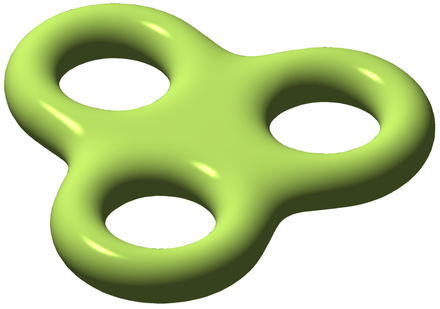
\includegraphics[scale = 1]{RiemannSurface}
**** Riemann Surface of genus 3, from Wikimedia ****

This definition does not apply to curves over fields other than $\CC$, and doesn't relate the genus to the algebra of the curve. However, we can relate the topological genus of a curve directly to its topological Euler characteristic. Since $C$ is topologically compact, connected, and oriented, we have
$H^{0}(C; \ZZ)=H^{2}(C; \ZZ) = \ZZ$, so:
$
\chi_{top}(C) = 2-2g.
$
By the Hopf index theorem, the topological Euler characteristic is the degree of the tangent sheaf, or equivalently, minus the degree of the cotangent sheaf $\omega_{C}$; that is, $\deg K_{C} = 2g-2$, and thus
$$
g(C) = \frac{\deg(K_C)}{2} + 1.
$$
This formula serves to define the genus of a smooth projective curve over any field. 
Other characterizations of the genus require more machinery to establish. We will state some here, and use  tools from the following section to prove the equivalences.

\begin{enumerate}

\item\label{pa}
$
g(C) = 1 - \chi(\cO_C). 
$

\item\label{genus Hilbert} If $C \subset \PP^r$ is a smooth curve of degree $d$  with homogeneous coordinate ring
$S_C$, then for sufficiently large $d$ the function $m \mapsto h_C(m) := \dim_\CC (S_C)_m$ is equal to a linear function
$$
p_C(m) =  dm - g + 1,
$$
so $g(C) = dm+1-p_C(m)$. 

\item\label{genus 1forms} $g(C)$ is the dimension of the vector space of regular 1-forms (that is, global sections of the
canonical sheaf) on $C$.
\end{enumerate}

\subsection{The Riemann-Roch Theorem}

To prove that these formulas for the genus are correct, we use \trr and Serre duality~\ref{sd} (sometimes called Kodaira-Serre duality, since Kodaira was responsible for the analytic version.)

\begin{theorem}[Riemann-Roch Theorem]\label{RR}
 If $C$ is a smooth, connected projective curve of genus $g$, and $D$ a divisor of degree $d$ on $C$ then
$$
h^0(D) = d - g + 1 + h^0(K_C - D).
$$
\end{theorem}

For example, if we take $D=0$, this tells us that $h^0(K) = g$, proving the characterization~(\ref{genus 1forms}) above. Using this and \trr for $D=K$
we get $\deg K = 2g-2$. Also, since $h^0(D) = 0$ for any divisor $D$ of negative degree, the formula gives the dimension of $h^{0}(D)$ when $\deg D$ is large:

\begin{corollary}\label{nonspecial RR}
For any divisor $D$ of degree $d$ we have
$$
h^0(D) \geq d - g + 1,
$$
with equality if $d > 2g-2$.
\end{corollary}
This was the theorem originally proven by Riemann; his student Roch supplied the correction term $h^0(K_C - D)$ for divisors of lower degree.
The dimension $h^0(K_C-D) = h^1(D)$ was called the \emph{superabundance} of $D$.

Corollary~\ref{nonspecial RR} and Proposition~\ref{very ample} together show that all high degree divisors come from hyperplane sections in 
suitable embeddings:

\begin{corollary}\label{degree 2g+1 embedding}
Let $D$ be a divisor of degree $d$ on a smooth, connected projective curve of genus $g$. If $d \geq 2g$, the complete linear series $|D|$ is base point free; and if $d \geq 2g+1$ the associated morphism $\phi_D : C \to \PP^{d-g}$ is an embedding, so that
$D$ is the preimage of the intersection of $C$ with a hyperplane in $ \PP^{d-g}$.
\end{corollary}

Since the complement of a hyperplane in projective space is an affine space, we get an affine embedding result too:

\begin{corollary}
 If $C$ is any smooth, connected projective curve and $\emptyset \neq \Gamma \subset C$ a finite subset then $C \setminus \Gamma$ is affine.
\end{corollary}
\begin{proof}
Let $D$ be the divisor defined by $\Gamma$. By Corollary~\ref{degree 2g+1 embedding} a high multiple of $D$ is very ample,
and gives an embedding $\phi: C\to \PP^n$ such that the preimage of the intersection of $C$ with some hyperplane $H$
is a multiple of $D$. It follows that $C\setminus \Gamma$ is embedded in $\AA^n = \PP^n\setminus H$.
\end{proof}
 
We can  use Corollary~\ref{nonspecial RR} to determine the Hilbert polynomial of a projective curve. To do this, let $C \subset \PP^r$ be a smooth curve of degree $d$ and genus $g$, and consider the exact sequence of sheaves
$$
0 \rTo \cI_{C/\PP^r}(m) \rTo \cO_{\PP^r}(m) \rTo \cO_C(m) \rTo 0
$$
and the corresponding exact sequence
$$
 H^0(\cO_{\PP^r}(m)) \rTo^{\rho_m} H^0(\cO_C(m)) \rTo H^1(\cI_{C/\PP^r}(m)) \rTo 0.
$$

The \emph{Hilbert function} $h_C$ of $C$  is defined by
$$
h_C(m) = \dim_{\CC} (S_{C})_{m} = \rank(\rho_m).
$$
By Theorem~\ref{Serre vanishing} we have $H^1(\cI_{C/\PP^r}(m)) = 0$ for large $m$, so $h_{C}(m) = h^0(\cO_C(m))$ for large $m$, which, by the Riemann-Roch theorem, equals $md-g+1$, again for large $m$. Thus, the Hilbert polynomial of $C \subset \PP^r$ is $p_C(m) = dm-g+1$, establishing the characterization~(\ref{genus Hilbert}).
 
The Riemann-Roch formula does \emph{not} give us a formula for the dimension $h^0(D)$ when $h^0(K_C - D)>0$; such divisors $D$ are called \emph{special divisors}. The existence or non-existence of divisors $D$ with given $h^{0}(D)$ and $h^{1}(D)$ often serves to distinguish one curve from another, and will be an important part of our study.


\subsection{Proof of Theorem~\ref{RR} from Theorem~\ref{sd}.}

If, following~\ref[Chapter IV]{H} we take the definition of the genus of  a smooth connected curve $C$ to be $h^1(\sO_C)$ (so that $g = h^0(K_C)$ becomes a Corollary of Theorem~\ref{sd}), then it is easy to establish the following form of the Riemann-Roch Theorem:

\begin{corollary}
 If $C$ is a smooth, connected projective curve and $D$ is a divisor on $C$ then
$$
\chi(\sO_C(C)) := h^0(D) - h^1(D) = d-g+1
$$
or in other words, for any invertible sheaf $\cL$ of degree $d$ on $C$,
$$
\chi(\cL) = d-g+1.
$$
\end{corollary}
\begin{proof}
 Taking $D=0$ the statement becomes $h^0(\sO) - h^1(\sO) = 1-g$, which is our definition of $g$. On the other hand,
for any divisor $D$ on $C$ and any point $p \in C$ we have an exact sequence of sheaves
$$
0 \to \cO_C(D-p) \to \cO_C(D) \to \frac{\cO_C(D)}{\gm_{C,p}\cO_C(D)} \to 0
$$
Since $\cO_C(D)$ is locally isomorphic to $\sO_C$ we see that $\cO_C(D)/\gm_{C,p}\cO_C(D)\cong \kappa(p)$ is a sky-scraper sheaf of dimension 1, concentrated at $p$,
and thus has Euler characteristic 1. 

Thus the Riemann-Roch Theorem for $\cO_C(D)$ is equivalent to the Riemann-Roch Theorem for $\cO_C(D-p)$. Since any divisor can be obtained from 0 by adding and subtracting points, the Riemann-Roch formula for an arbitrary $\cL$ follows from the special case $\cL = \cO_C$ with which we began.
\end{proof}


\subsection{Arithmetic genus and geometric genus}
In this section, we'll deal with a  curve $C_0$ that is assumed to be reduced and irreducible, but not necessarily smooth.
Given $C_0$ there is a unique normalization morphism $\nu: C \to C_0$, and thus $C_0$ is birational to a unique
smooth curve. The genus of $C$ is called the \emph{geometric genus} of $C_0$.

Most of the results of this book have analogues for singular curves, but this is a topic beyond our scope; for us, the questions are about smooth curves, with singular curves appearing as a useful adjunct, for example in Chapter~\ref{PlaneCurveChapter}.

Applied to a possibly singular or even non-reduced 1-dimensional projective scheme, the formula~\ref{pa} and the equivalent~\ref{genus Hilbert}, define
what is called the \emph{arithmetic genus} $p_a(C)$. 

We can relate the arithmetic and geometric genera of $C_0$ using the map of sheaves
$$
\cO_{C_0} \to \nu_*\cO_C.
$$
This is injective; the cokernel sheaf will be a skyscraper sheaf supported on the singular points of $C_0$. Denoting this sheaf by $\cF$, we have an exact sequence
$$
0 \to \cO_{C_0} \to \nu_*\cO_C \to \cF \to 0.
$$

\fix{insert statement of Leray here. It will be used again in the Plane curve chapter}

The normalization map $\nu: C \to C_0$ is finite, so that the direct images $R^i\nu_*\cO_C$ vanish for $i > 0$; it follows from the Leray spectral sequence that $\chi(\nu_*\cO_C) = \chi(\cO_C)$. Thus
$$
p_a(C_0) - g(C) =  \chi(\cO_{C}) -   \chi(\cO_{C_0}) = \chi(\cF) = h^0(\cF);
$$ 
in other words, the difference between the arithmetic and geometric genera of $C_0$ is the sum of the vector space dimensions of the stalks of $\cF$; colloquially, it's the number of linear conditions a function $f$ on $C$ has to satisfy to be the pullback of a function from $C_0$. The length of the stalk of $\cF$ at a particular singular point $p \in C_0$ is called the \emph{$\delta$-invariant} $\delta_p$ of the singularity; to rephrase the statement above in these terms, we have:
$$
p_a(C_0) - g(C) = \sum_{p \in (C_0)_{sing}} \delta_p
$$ 

The $\delta$ invariant is easy to compute in simple cases:
\begin{enumerate}

\item (nodes) If $p \in C_0$ is a node, with points $r,s \in C$ lying over it, the condition for a function $f$ on $C$ to descend is simply that $f(r)=f(s)$; this is one linear condition so $\delta_p = 1$.

\item (cusps) If $p \in C_0$ is a cusp, with  $r \in C$ lying over it, the condition for a function $f$ on $C$ to descend is simply that the derivative $f'(r)=0$; again, this is one linear condition so $\delta_p = 1$.

\item (tacnodes) Suppose now that $p \in C_0$ is a \emph{tacnode}, that is, $C_0$ has two smooth branches at $p$ simply tangent to one another. There will be two points $r, s \in C$ lying over it, and the condition for a function $f$ on $C$ to descend is that in terms of suitable local coordinates both $f(r)=f(s)$ and $f'(r)=f'(s)$.  This represents two linear conditions, so $\delta_p = 2$.

\item (planar triple points) An ordinary triple point $p \in C_0$ of a plane curve is a singularity consisting of three smooth branches meeting pairwise transversely, such as the zero locus of $y^3-x^3$. There will be three points $r,s,t \in C$ lying over $p$, and certainly a necessary condition for a function $f$ on $C$ to descend is that $f(r)=f(s)=f(t)$---two linear conditions. But there's a third, less obvious linear condition: in order for $f$ to descend, the derivatives $f'(r), f'(s), f'(t)$ have to satisfy a linear condition---a reflection of the fact that a function on $C_0$ cannot vanish to order 2 on each of two branches without vanishing to order 2 along the third as well. Thus $\delta_p = 3$

\item (spatial triple points) We will be concerned in what follows only with planar singularities, but spatial triple points provide a useful contrast to the last example. A spatial triple point is a singularity consisting of three smooth branches, with linearly independent tangent lines, so that its Zariski tangent space is 3-dimensional. An example would be the union of the three coordinate axes in $\AA^3$.

In this case, in contrast to case of the planar triple point, the condition that $f(r)=f(s)=f(t)$ is both necessary and sufficient for $f$ to descend, and thus  $\delta_p=2$.

\end{enumerate}


\subsection{Clifford's theorem}

While the Riemann-Roch Theorem gives a lower bound for the dimension of a linear series, $r(\sL) := h^0(\sL)-1 \geq \deg \sL -g$, Clifford's Theorem
gives an upper bound. If $\deg \sL>2g-2$, then the Riemann-Roch inequality becomes an equality, so it is enough to treat the case $\deg \sL \leq 2g-2$.
To state the sharpest form, we define a curve $C$ of genus $\geq 2$ to be \emph{hyperelliptic} if there exists a $g^1_2$ on $C$; that is an
invertible sheaf $\cL$ of degree $2$ with 2 independent global sections or, equivalently, a morphism $C\to \PP^1$ of degree 2. We will see in Chapter~\ref{genus 2 and 3 chapter} that such a sheaf would be unique, and $h^0(\cL) = 2$, and that such curves have extremely special properties.


\begin{theorem}\label{Clifford}
Let $C$ be a curve of genus $g$ and $\cL$ a line bundle of degree $d \leq 2g-2$. Then
$$
r(\cL) \leq \frac{d}{2}.
$$
Moreover, if  equality holds then we must have either
\begin{enumerate}
\item $d=0$ and $\cL = \cO_C$;
\item $d = 2g-2$ and $\cL = K_C$; or
\item $C$ is hyperelliptic, and $|\cL|$ is a multiple of the $g^1_2$ on $C$.
\end{enumerate}
\end{theorem}

The proof of the inequality will follow easily from a basic result about the addition of linear series, defined as follows:
$\cD = (\cL,V)$ and $\cE = (\cM, W)$ be two linear series on a curve $C$. By the \emph{sum} $\cD + \cE$ of $\cD$ and $\cE$, we will mean the pair 
$$
\cD + \cE = (\cL \otimes \cM, U) 
$$
where $U \subset H^0(\cL \otimes \cM)$ is the subspace generated by the image of $V \otimes W$, under the multiplication/cup product map $H^0(\cL) \otimes H^0(\cM) \to H^0(\cL \otimes \cM)$---in other words, it's the subspace of the complete linear series $|\cL\otimes \cM|$ spanned by divisors of the form $D+E$, with $D \in \cD$ and $E \in \cE$.
 
\begin{proof}
If $\cD$ and $\cE$ are two nonempty linear series on a curve $C$, then
$$
\dim(\cD + \cE) \geq \dim \cD + \dim \cE.
$$
To see this, we observe that to say $\dim \cD \geq m$ means exactly that we can find a divisor $D \in \cD$ containing any given $m$ points of $C$; since $\cD + \cE$ contains all pairwise sums $D + E$ with $D \in \cD$ and $E \in \cE$, we can certainly find a divisor $F \in \cD + \cE$ containing any given $\dim \cD + \dim \cE$ points of $C$.

The proof of the inequality in Clifford's Theorem follows  by applying this observation to the pair $|\cL|$ and $|K_C\otimes \cL^{-1}|$: by 
the Riemann-Roch Theorem, we have
$$
r(K_C\otimes \cL^{-1}) = r(\cL) +g - d - 1
$$
and so we deduce that
$$
g = r(K_C) + 1 \geq r(\cL) + r(K_C\otimes \cL^{-1}) + 1 \geq 2r(\cL) +g - d;
$$
hence $r(\cL) \leq d/2$.

For the proof of the second half of Clifford's Theorem, we will use a basic fact about the geometry of hyperplane sections of a curve in projective space (Proposition~\ref{monodromy of hyperplane section}); we give the proof after proving that result.
\end{proof}



\section{The canonical morphism}

We will generally begin to study the invertible sheaves on a smooth curve $C$ by studying the complete linear series associated to the canonical divisor $|K|$ and the \emph{canonical map}
 $\phi_K : C \to \PP^{g-1}$. 
 
 In the case $g=0$ the canonical sheaf has degree 0 and since it has nonzero global sections, 
 $\omega_C = \sO_C$, and $K_C = 0$. Thus we restrict our attention to smooth curves $C$ of genus $g\geq 2$. We will see
 that the canonical series is then base-point free, so $|K|$ defines a morphism.

Recall that a curve of genus $\geq 2$
is said to be \emph{hyperelliptic} if there exists a morphism $f: C \to \PP^1$ of degree 2. 


\begin{theorem}\label{canonical series is very ample}
If $C$ is a smooth curve of genus $\geq 2$ then the canonical morphism $\phi_K : C \to \PP^{g-1}$ is an embedding if and only if $C$ is not hyperelliptic. 
\end{theorem}

The image of the canonical morphism of a non-hyperelliptic curve of genus $g>2$ is called a \emph{canonical curve}.

\begin{proof}
By Corollary~\ref{degree 2g+1 embedding} we have to show that for any pair of points $p, q \in C$ we have
$$
h^0(K_C(-p-q)) = h^0(K_C)-2 = g-2.
$$
Applying \trr we see this fails if and only if $h^0(\cO_C(p+q)) \geq 2$ for some $p,q \in C$. By Lemma~\ref{deg 2 morphism}, this implies that $C$ is hyperelliptic.
\end{proof}

\begin{lemma}\label{deg 2 morphism}
Let $C$ be a smooth, projective curve of genus $g\geq 2$. If $C$ has an invertible sheaf $\cL$ of degree 2 with two independent sections, then
$|\cL|$ defines a morphism of degree 2 to $\PP^{1}$, and $C$ is hyperelliptic. In particular, if $g(C) = 2$ then the canonical series $|K_{C}|$ defines a 2 to 1 morphism to $\PP^{1}$, so $C$ is hyperelliptic.
\end{lemma}

\begin{proof}
If $\cO_C(p+q)$ has two independent sections and has $d$ basepoints, then it defines a morphism of degree $2-d$ to $\PP^1$. Since $C$ is not rational,
we must have $d=0$, proving the first statement. 
\end{proof}

\subsection{The geometric Riemann-Roch theorem}

If $C$ is a nonhyperelliptic curve, embedded in $\PP^{g-1}$ by its canonical series and  $D = p_1+\dots + p_d$ is a divisor consisting of $d$ distinct points, we will write $\overline D$ be the span of the points $p_i \in C \subset \PP^{g-1}$. Since the hyperplanes in $\PP^{g-1}$ containing $\{p_1,\dots,p_d\}$ correspond (up to scalars) to sections of $K_C$ vanishing at all the points $p_i$, we see that
$$
h^0(K_C-D) = g - 1 - \dim \overline D = \codim \overline D \subset \PP^{g-1}
$$
Plugging this into the Riemann-Roch formula, we arrive at the statement
$$
r(D) = d - 1 - \dim \overline D;
$$
or in other words, the dimension of the linear series $|D|$ in which the divisor $D$ moves is equal to the number of linear relations on the points $p_i$ on the canonical curve. Thus, for example, if $D = p_1+p_2+p_3$, we see that $D$ moves in a pencil if and only if the points $p_i$ become collinear under the canonical morphism.

We can extend this statement to the case of arbitrary effective divisors $D$ on any smooth curve if we define our terms correctly. To do this, suppose $f : C \to \PP^d$ is any morphism, and $D \subset C$ any divisor. We define the \emph{span} of  $f(D)$ to be the intersection
$$
\overline{f(D)} = \bigcap_{H \mid f^{-1}(H)\supset D} H 
$$
of all hyperplanes in $\PP^d$ whose preimage in $C$ contains $D$. The argument above applies to prove:

\begin{theorem}[Geometric Riemann-Roch Theorem]\label{geometric RR}
If $C$ is any curve of genus $g \geq 2$,  $\phi : C \to \PP^{g-1}$ its canonical morphism and $D \subset C$ any effective divisor of degree $d$, then
$$
r(D) = d - 1 - \dim \overline{\phi(D)}.
$$
\end{theorem}
 
 \section{Canonical curves are projectively normal}\label{Noether theorem section}

When we analyze the embedding of a curve $C\subset \PP^n$ we generally ask first whether $C$ is contained in any low-degree
hypersurfaces, and if so how many, in the sense of the dimension $(I_C)_d)$ the degree $d$ part of the homogeneous ideal of $C$.
From the long exact sequence in cohomology
$$
0\to H^0(\sI_{C/\PP^n}(d)) \to H^0(\sO_{\PP^n}(d)) \to H^0(\sO_C(d)) \to H^1(\sI_{C/\PP^n}(d)) \to H^1(\sO_{\PP^n}(d)) \to\cdots
$$
together with the identification of $H^0(\sO_{\PP^n}(d))$ with the vector space of degree $d$ forms on $\PP^n$, and  the fact that
 $H^1(\sO_{\PP^n}(d)) = 0$ for all $n>1$ and all $d\geq 0$, we see that
 $$
 \dim (I_C)_d = h^0(\sI_{C/\PP^n}(d)) = h^0(\sO_{\PP^n}(d)) - h^0(\sO_C(d)) + h^1(\sI_{C/\PP^n}(d)).
$$
If $d$ times the degree of $C$ is $>2g-2$, the the Riemann-Roch Theorem tells us the value of
 $h^0(\sO_C(d))$, and thus a lower bound for $ \dim (I_C)_d$, but if, in addition, the map
 $H^0(\sO_{\PP^n}(d) \to H^0(\sO_C(d))$ is surjective (or equivalently $h^1(\sI_{C/\PP^n}(d))=0$),
 then we get $ \dim (I_C)_d$ exactly.
 
 
\begin{definition} An embedding of a smooth curve
$C\subset \PP^n$ is said to be \emph{projectively normal} or \emph{arithmetically Cohen-Macaulay} if all the maps $H^0(\sO_{\PP^n}(d)) \to H^0(\sO_C(d))$ are surjective,
or equivalently $h^1(\sI_{C/\PP^n}(d))=0$ for all $d\geq 0$.
\end{definition}
 
 
\begin{remark}
 Smooth varieties are of course normal and Cohen-Macaulay in the sense that their local rings have these properties. The condition of ``projective normality'' is equaivalent, by Serre's Criterion (see for example~\cite[Section 11.2]{Eisenbud1995}), to the normality of the homogeneous coordinate ring of $C$. In the case of smooth curves, this is equivalent to the condition that the homogeneous coordinate
ring is Cohen-Macaulay, whence the term \emph{arithmetically Cohen-Macaulay} (sometimes also, confusingly, called
\emph{projectively Cohen-Macaulay}.
\end{remark}

 The criterion has two parts, which are interesting separately: A local or graded ring is normal if it is nonsingular in
codimension 1; and
locally of depth $\geq 2$ in codimension $\geq 2$ (\cite[Theorem 11.5]{Eisenbud1995}) In the case of the homogeneous coordinate ring of a curve, 
the first condition means that the curve is nonsingular and the second means that $h^1(\sI_{C/\PP^n}(d))=0$ for all $d$.
It follows that for any very ample invertible sheaf $\sL$ on a smooth curve $C$, the ring 
$$
R(C, \sL) := \bigoplus_{m=0}^\infty H^0(\sL^m)
$$
is the normalization of the homogeneous coordinate ring in the embedding of $C$ by $|\sL|$.

\begin{example}\label{rnc is projectively normal}
For $d\geq 1$ the rational normal curve $C\subset \PP^d$ of degree $d$ is projectively normal. 
We have $H^0(\sO_{\PP^1}(md))  = \CC[s,t]_{md}$. Th natural natural map
$$
\CC[x_0,\dots,x_d] \to\bigoplus_{m = 0}^\infty H^0(\sO_{\PP^1}(md)));\quad x_0,\dots, x_d \mapsto s^d,s^{d-1}t,\dots, t^d
$$ 
is surjective since every monomial of degree $md$ can be written as a monomial in  
the elements $s^d,s^{d-1}t,\dots, t^d$, and the ring is normal (Exercise~\ref{normality of RNC}).
\end{example}

We will now show that the canonical image of a smooth curve is always projectively normal. When the curve is hyperelliptic,
the canonical image is the rational normal curve, treated above, so we may assume that the curve $C$ is embedded
by $|K_C|$ as a smooth curve in $\PP^{g-1}$.

To do this we will make use of an auxiliary construction, a \emph{simple $(g-4)$-secant $(g-3)$-plane.}

\begin{lemma}\label{simple secant}
 If $C\subset \PP^n$ is a smooth nondegenerate curve, $n\geq 3$, and $m\leq n-1$, then the linear span $L := \overline{p_1,\dots, p_m}$
 of $m$ general points of $C$ is a simple $m$-secant; that is, a plane of dimension $m-1$ such that
 $C\cap L = \{p_1,\dots,p_m\}$ scheme-theoretically.
 \end{lemma}
 
\begin{proof}
By Lemma~\ref{general position lemma} the points of a general hyperplane section are in linearly general position.
\end{proof}

The following was proven, for smooth curves, by Max Noether, Emmy's father.

\begin{theorem}\label{canonical curves are ACM}
If $C\subset \PP^{g-1}$ is the canonical image of a smooth curve of genus $\geq 2$ then the natural maps
$\HH^0(\sO_{\PP^{g-1}}(m) \to \HH^0(\sO_C(m)$
are surjective for all $m\in \ZZ$; equivalently,
$\HH^{1}(\sI_{C/\PP^{g-1}}(m)) = 0$ for all $m\in \ZZ$.
\end{theorem}
 
We will follow Schreyer's presentation of the proof from~\cite{Schreyer}, which has the advantage that it applies to a wide range of singular
curves as well. 
 
   
\begin{proof} 
One sees the equivalence of the two statements from the long exact sequence in cohomology coming from the sequences
$$
0\to sI_{C/\PP^{g-1}} \to\sO_{\PP^{g-1}} \to \sO_C \to 0 
$$
after tensoring with $\sO_{\PP^{g-1}}(m)$.


The invertible sheaf $\sO_C(-m)$ has negative degree, and thus no nonzero global sections for $m<0$.
For $m=0,1$ the surjectivity of  $\HH^0(\sO_{\PP^{g-1}}(m) \to \HH^0(\sO_C(m)$ is immediate from the hypothesis that $C$ is
the image of a map corresponding to a complete linear series.

If
$g=2$ then $C$ is a line, and the result is trivial, so we may assume $g\geq 3$.

%Also, if $g=3$ then $C$ is a plane quartic,
%and $\sI_{C/\PP^{g-1}} = \sO_{\PP^2}(-4)$. Since $H^1(\sO_{\PP^n}(d)) = 0$ for all $n>1$ and all $d$, the Theorem is true
%in this case. Thus we may assume $g\geq 4$.

By Lemma simple secant, $C$ in has a  simple $g-3$-dimensional $g-2$ secant plane $\Lambda$. Write
$\Lambda\cap C = \{p_1,\dots, p_{g-2}\}$. Choose linear forms $x_1,\dots, x_{g-2}$ on $\PP^{g-1}$ such that
$x_i$ vanishes on $p_j$ if and only if $i=j$. 

To simplify the notation, let $D$ be the divisor $p_1+\cdots+p_{g-2}$.
The sheaf $\sO_C(K_C)$, restricted to any finte set is trivial,
so the quotient 
$$
\frac{\sO_C(K_C-D)}{\sO_C(mK_C-D)}
$$
is generated by $x_1^m,\dots, x_{g-2}^m$ for every $m\geq 1$.
Thus it suffices to show that the maps
$$
\HH^0(K_C-D) \otimes \HH^0(\sO_C((m-1)K_C)) \to \HH^0(\sO_C(mK_C -D)
$$
are surjective for every $m\geq 2$.

By the geometric Riemann-Roch theorem, divisor $K_C-D$ move in a base-point free pencil; that is
$V = \HH^0(K_C-D) = \CC^2$, and setting $\sL = \sO_C(K_C-D)$ for simplicity,
 the linear series $(\sL, V)$ is base-point free. 

The following argument is sometimes called the \emph{base-point-free pencil trick}: Choose sections $\sigma_1, \sigma_2$ that
generate the 2-dimensional vector space $V$, and consider the complex of sheaves
$$
0\to \wedge^{2} V\otimes \sL^{-1} \rTo^{
\begin{pmatrix}
 \sigma_2\\-\sigma_1
\end{pmatrix}}
 V\otimes \sO \rTo^{
\begin{pmatrix}
 \sigma_2&\sigma_2
\end{pmatrix}}
 \sL \to 0. \quad (*)
$$
Locally at a point $p$ we may identify $\sigma_1,\sigma_2$ with functions in the local ring $R := \sO_{C,,p}$
and rewrite the complex as
$$
0 \to R \rTo^{
\begin{pmatrix}
 \sigma_2\\-\sigma_1
\end{pmatrix}}
R^2 \rTo^{
\begin{pmatrix}
 \sigma_2&\sigma_2
\end{pmatrix}}
R \to 0. \quad (**)
$$
Since $p$ is not a basepoint of the pencil, with this identification
 $(\sigma_1, \sigma_2)\subset R$ is the unit ideal, so the  sequence $(**)$ is exact, and
 thus the sequence $(*)$ of sheaves is exact too. 
 
 We now tensor the sequence $(*)$ with $\sO_C((m-1)K)$ obtaining an exact sequence
 $$
0\to \wedge^{2} V\otimes \sO_C((m-2)K+D) \rTo V\otimes \sO_C((m-1)K) \rTo \sO_C(mK-D) \to 0.
$$
By the argument at the beginning of the proof, it suffices to show that this induces an exact sequence
on global sections for all $m\geq 2$.

For $m = 2$, we see, again by the geometric Riemann-Roch theorem, that $h^0(\sO_C(D)) = 1$,
while $\dim_\CC(V\otimes \HH^0(\sO_C(K) )= 2g$. Since $\deg(2K-D) = 3g-2>2g-2$, the Riemann-Roch
theorem gives $h^0(\sO_C(2K-D)) = 2g-1$. Since the sequence on cohomology is automatically left-exact,
this dimension computation shows that it is exact.

Finally, for $m>2$ the degree of $(m-2)K+D$ is $>2g-2$, so $\HH^1(\sO_C((m-2)K+D))= 0$ so again we see
that the required sequence is exact, completing the proof.
\end{proof}

\begin{corollary}\label{canonical hilbert function}
If $C\subset \PP^{g-1}$ is a canonical curve with a simple $g-3$-secant, then the Hilbert function of the homogeneous coordinate ring $S_{C}$ of  $C$ depends only on $g$, and is given by:
$$
\dim({S_{C}})_{d} = h^{0}(\cO_{C}(d)) = 
\begin{cases}
 0 &\mbox {if } d<0\\
 1 & \mbox {if }  d=0\\
 g & \mbox {if }  d=1\\
 (2n-1)g+1 & \mbox {if }  d>1\\
\end{cases}
$$
\end{corollary}
\begin{proof}
Theorem~\ref{canonical curves are ACM} implies, in particular, that the homogeneous coordinate ring of $C$ can be identified with 
$\oplus_{n\in \ZZ}\HH^0\sO_C(n)$.  
\end{proof}

 \section{A bit about surfaces}
 We will often analyze curves  on a smooth surface; here are a few results that will be useful. We refer to~\cite[Chapter V]{Hartshorne1977}
 and~\cite[Chapter I]{Beauville} for proofs.
 
 We suppose for this section that $X$ is a smooth projective surface.
 We define $\Pic(X)$ to be the group whose elements are invertible sheaves on $X$.
When two divisors $D,E$ on $X$ meet transversely we define $D\cdot E$ to be the number of points in which they meet. If they have no common
components, we can still define a non-negative intersection multiplicity $m_X(D,E,p)$ at each point $p$, and then set
$$
D\cdot E = \sum_p m_X(D,E,p).
$$
Over the complex numbers each codimension 1 subvariety $D$ of $X$ has a fundamental class
$[D]\in H^2(X, \ZZ)$ and the product is the cup product with values in $H^4(X,\ZZ)$, which is $\ZZ$ since $X$ is compact and orientable. Thus
there is an extension of the product to the cases where $D,E$ have common components. From a geometric point of view, we may choose an
appropriate $C^\infty$
normal vector field along $E$ and define $E'$ by ``pushing'' $E$ out slightly along the direction of this field, until $D$ and $E'$ are transverse,
and the intersections can be computed in the usual way. It should be noted that such intersection numbers can be either positive or negative,
since they depend on the relative orientations of $D$ and $E'$ at the intersection points; this is in contrast to the case when $D$ and $E$
themselves meet properly; in this case the fact that the complex numbers are canonically oriented makes the intersection number non-negative.

The intersection product can also be defined algebraically, over any field: Setting $\sL := \sO_X(C)$ and
$\sM := \sO_X(D)$ to simplify the notation, we set 
$$
D\cdot E = \chi(\sO_X)-\chi(\sL^{-1}) -\chi(\sM^{-1}) -\chi(\sL^{-1}\sM^{-1}) 
$$
\begin{theorem} The pairing $(D,E) \mapsto (D.E)$ is the unique bilinear map
$\Pic(X) \times \Pic(X) \to \ZZ$ extending the case of intersections of two transverse curves on $X$. 
\end{theorem}

A frequent use of the the intersection pairing is to compute the (arithmetic) genus of a curve on a surface,
a result called the adjunction formula.

\begin{theorem}[Adjunction Formula]\label{adjunction formula}
If $C$ is a curve lying on a smooth surface $X$ then 
$$
\omega_C = \omega_X \otimes \sO_X(C) \otimes \sO_C.
$$
In particular \label{genus formula}
$$
p_a(C) = \frac{(K_X+C)\cdot C}{2} +1
 $$
\end{theorem}

We will frequently be interested in curves on quadrics in $\PP^3$, and we can spell out the
intersection theory on these surfaces very concretely; see for example~\cite[****]{Hartshorne1977}.
We will treat them and the curves on them in detail in Section~\ref{curves on scrolls} as part of the larger family of 2-dimensional rational normal scrolls; for
now we sketch the situation as an example of the theory of this section. 

\begin{example}[Quadrics in $\PP^3$]\label{Div of quadric}
 
Quadric surfaces $S$ in $\PP^3$ are classified by their rank:
\begin{itemize}
\item A quadric of rank 2 is the union of two planes; it cannot contain an nondegenerate irreducible curve
\item A rank 3 quadric $S$ is a cone over a plane conic. Suppose that $C$ is a smooth,
curve on such a quadric:
\begin{itemize}
\item  If $C$  does
not pass through the vertex then it is the intersection of the quadric with a hypersurface of some
degree $d$. In this case $C$ has degree $2d$ and genus $(d-1)^2$. 
 \item if $C$ passes through the vertex, then $C$ lies in the divisor class of a line through the origin plus the intersection of $S$ with a hypersurface of some degree $d$. In this case $C$ has degree $2d+1$ and 
 genus $d(d-1)$. 
\end{itemize}

%If  it contains smooth irreducible curves that do not pass through the vertex of the cone, and smooth irreducible curves that of
%degree $2d$ that are intersections of $S$ with hypersurfaces of degree $d$; and smooth 
%irreducible curves of degree $2d+1$ that 

\item A quadric of rank 4 is nonsingular, and is isomorphic to $\PP^1\times \PP^1$.


\item The Picard group of $\PP^1\times \PP^1$ is $\ZZ\oplus \ZZ$, generated by the 
classes of the lines $\{p\}\times \PP^1$ and $\PP^1\times \{p\}$, where $p\in \PP^1$
is any point. These lines have self-intersection 0, and meet transversely in a point,
so the intersection pairing is given by $(a,b)\cdot(c,d) = ad+bc$. From the adjunction formula
applied to the classes of the lines $(1,0)$ and $(0,1)$ we that the canonical
class is $(-2,-2)$, and thus the arithmetic genus of a curve of type $(a,b)$ is thus
$$
\left(((a,b)+(-2,-2))\cdot (a,b)\right)/2 +1 = (a-1)(b-1).
$$

\item Writing $\pi_1, \pi_2$ for the two projections of
$\PP^1\times \PP^1 \to \PP^1$, the sheaf 
$$
\sL := \sO_{\PP^1\times \PP^1}(a,b) = \pi_1^*\op1a \otimes \pi_2^*\op1b
$$
has cohomology given by the K\"unneth formula, for example
\begin{align*}
 H^0(\sL) &= H^0(\op1a)\otimes H^0(\op1b) \hbox{ and thus }\\
 h^0(\sL) &= (a+1)(b+1) \hbox{ if } a\geq 0, b\geq 0.
\end{align*}

\item Any smooth quadric surface $S\subset \PP^3$ is the 
image of $\PP^1\times \PP^1$ embedded by the complete linear series
$|\sO_{\PP^1\times \PP^1}(1,1)|$ and thus contains two families of lines. 
A curve in the class $(a,b)$ thus has degree $(a,b)\cdot(1,1) = a+b$. 
\end{itemize}
\end{example}

Often we wish to compute the dimension of the space of sections of an invertible sheaf, but
as with the case of curves, the Euler characteristic is more accessible:

\begin{theorem}[Riemann-Roch for surfaces] Let $\sL$ be an invertible sheaf on a smooth surface $S$.
the Euler characteristic $\chi(D) := h^0(\sL)-h^1(\sL)+h^2(\sL)$, where $\sL = \sO_S(D)$, is given by
$$
\chi(D) = \chi(\sO) + \frac{(D-K_S)\cdot D}{2}+1
$$
\end{theorem}

%\fix{Possible addition:  the Hodge Index theorem as corollary. This could be used to prove finiteness of the automorphism group of a curve following Hartshorne V Ex. 1.11, perhaps in place of the proof now in the inflections chapter.}

It is useful to know what happens under mappings of surfaces, particularly the case of the mapping
corresponding to blowing up a point.

\begin{theorem}
If $\pi: X \to Y$ is a birational map of smooth surfaces, then the pullback map on divisors
preserves the intersection pairing. If $X$ is the blowup of $Y$ at a point $p$, with exceptional
divisor $E = \pi^{-1}(p)$ then:

\begin{enumerate}
 \item $\Pic X =\pi^*(\Pic Y) \oplus \ZZ E$.
\item The canonical class on $X$ is given by $K_X = \pi^*(K_Y)+E$.
 \item The intersection pairing on $\Pic X$ is given by
 
\begin{itemize}
\item $\pi^*(D)\cdot\pi^*(D') = D.D'$ for all $D,D'\in \Pic Y$.
\item $\pi^*(D)\cdot E = 0$ for all $D\in \Pic Y$.
 \item $E\cdot E = -1$.
 \item $K_X\cdot E = -1$.
 \item If $C$ is a curve that has an $m$-fold point at $p$ then $\pi^{-1}(C)$ contains $E$ with multiplicity $m$.
 \end{itemize}
\end{enumerate}
\end{theorem}

Blowups occur frequently in the theory of surfaces, and are easy to characterize:
\begin{theorem}
If $E\subset X$ is a curve on a smooth projective surface $X$ and
 that $E^2 = E\cdot K_X = -1$ then $E$ can be ``blown down'' in the sense that
 $X$ is the blowup of a smooth surface $Y$ at a point $p\in Y$, and $E$ is the exceptional divisor.
\end{theorem}

\section{Exercises}

In the following series of exercises, we are going to be working with smooth projective curves associated to a given affine curve $C^\circ := V(f(x,y)) \subset \AA^2$; this is the unique smooth projective curve containing the normalization of $C^\circ$ as a Zariski dense open subset.

\begin{exercise}
Let $C$ be the smooth projective curve associated to the affine plane curve $y^3 +x^3 = 1$, and let $\pi : C \to \PP^1$ be the map given by the rational function $x$.
\begin{enumerate}
\item Find the branch points and ramification points of $\pi$, and deduce that the genus of $C$ is 1.
\item For any two points $p, q \in C$ find the complete linear series $|p+q|$.
\item Find the (unique) map $\eta : C \to \PP^1$ of degree 2 such that $\eta((1,0)) = \eta((0,1))$, and determine the ramification points of $\eta$.
\item Show that $C$ is isomorphic to the smooth projective curve associated to the affine plane curve $y^2 +x^3 = 1$.
\end{enumerate}
\end{exercise}

For the next three exercises, let $C^\circ$ be the affine plane curve given as the zero locus of $y^2 - x^6 +1$, and let $C$ be the corresponding smooth projective curve. Note that the map $C^\circ \to \AA^1$ given by the projection $(x,y) \mapsto x$ extends to a map $\pi : C \to \PP^1$, expressing $C$ as a 2-sheeted cover of $\PP^1$ branched over the points $1, \zeta, \dots, \zeta^5$, where $\zeta$ is any primitive 6th root of unity. In addition, let $p$ and $q \in C$ be the two points lying over the point $\infty \in \PP^1$.

\begin{exercise}\label{hyperelliptic curve 1}
Let $C^\circ$ be the affine plane curve given as the zero locus of $y^2 - x^6 +1$, and let $C$ be the corresponding smooth projective curve. 

Show  that the map $C^\circ \to \AA^1$ given by the projection $(x,y) \mapsto x$ extends to a map $\pi : C \to \PP^1$, expressing $C$ as a 2-sheeted cover of $\PP^1$ branched over the points $1, \zeta, \dots, \zeta^5$, where $\zeta$ is any primitive 6th root of unity. Show that there are two distinct points $p$ and $q \in C$  lying over the point $\infty \in \PP^1$,
so that $C$ is unramified over $\infty$.

What is the genus of $C$?
\end{exercise}

\begin{exercise} With $C$ as in Exercise~\ref{hyperelliptic curve 1}:
\begin{enumerate}

\item Let $r_\alpha$ be the branch point over $\zeta^\alpha$. Show that
$$
p+q \sim 2r_\alpha \quad \text{and} \quad \sum_{\alpha = 0}^5 r_\alpha \sim 3p+3q.
$$

\item Find the vector space $\cL(D)$ where $D = r_0 + r_2 + r_4$, and find the (unique) divisor $E$ on $C$ such that $E + r_1 \sim r_0 + r_2 + r_4$.

\end{enumerate}

\end{exercise}


\begin{exercise}
With $C$ as in Exercise~\ref{hyperelliptic curve 1}:
Let $D$ be the divisor $D = p + q + r_0 + r_3$
\begin{enumerate}
\item Find the vector space $\cL(D)$.
\item Describe the map $\phi_{|D|} : C \to \PP^2$.
\item Find the equation of the image curve $\phi_{|D|}(C) \subset \PP^2$, and describe its singularities.
\end{enumerate}
\end{exercise}

The following exercises deal with the curve 
\begin{exercise}
Let $C$ be the smooth projective curve associated to the affine curve $y^3 = x^5 -1$. Note that the map $\pi : C \to \PP^1$ given by the function $x$ expresses $C$ as a cyclic, 3-sheeted cover of $\PP^1$, branched over the 5th roots of unity and the point at $\infty$. By way of notation, if we take $\eta = e^{2\pi i/5}$ a primitive 5th root of unity, we'll denote by $r_\alpha$ the point $(\eta^\alpha, 0) \in C$ lying over $\eta^\alpha$, and by $p$ the point lying over $\infty \in \PP^1$.

\begin{enumerate}
\item Verify that there is indeed a unique point $p \in C$ lying over $\infty \in \PP^1$, and the map has ramification index 2 at $p$. 
\item Show that the genus of $C$ is 4.
\item Establish the linear equivalences
$$
3p \sim 3r_\alpha \quad \text{and} \quad r_1+ \dots + r_5 \sim 5p.
$$
\item Find a basis for the space $H^0(K_C)$ of regular differentials on $C$.
\item Show that $C$ is not hyperelliptic.
\item Describe the canonical map $\phi_K : C \to \PP^3$ and find the equations of the image.
\item Let $D$ be the divisor $D = r_1+\dots+r_5$. Show that $h^0(K_C(-D)) = 1$; deduce that $r(D) = 2$, and find a basis for $H^0(\cO_C(D))$.
\item If $E = 3p$, show that $r(E) = 1$; that $|E|$ is the unique $g^1_3$ on $C$ and that $2E \sim K$.
\end{enumerate}
\end{exercise}


\begin{exercise}\label{gonality exclusion}
Show that a curve of genus $g \geq 3$ cannot be simultaneously hyperelliptic and a three-sheeted cover of $\PP^1$.
\end{exercise}


\begin{exercise}\label{here there be basepoints}
 Show that there is no non-constant morphism $\PP^r\to \PP^s$ when $s<r$ by showing that any nontrivial linear
 series of dimension $<r$ has a non-empty base locus.
\end{exercise}

\begin{exercise}
Extend the statement of Proposition~\ref{very ample} to incomplete linear series; that is, prove that the morphism associated to a linear series $(\cL, V)$ is an embedding iff
$$
\dim\big( V \cap H^0(\cL(-p-q))\big) = \dim V - 2 \quad \forall p, q \in C.
$$
\end{exercise}

\begin{exercise}
An automorphism of $\PP^r$ takes hyperplanes to hyperplanes. Deduce that it is given by the linear series
$\sV = (\sO_{\PP^r}(1), H^0(\sO_{\PP^r}(1)))$, and use this to show that $\Aut \PP^r = PGL(r+1)$. 
\end{exercise}

\begin{exercise}\label{projective automorphism}
In the circumstances above, the automorphism $\phi$ is induced by an automorphism of $\PP^r$ if and only if $\phi$ carries the invertible sheaf $\cO_{C}(1)$ to itself; that is, $\phi^*(\cO_{C}(1)) = \cO_{C}(1)$. In this case we say that the
\end{exercise}

\begin{exercise}
Show that normalization of the affine planar triple point $xy(x-y) = 0$ in $\AA^2$ is the disjoint union of three
affine lines, $\Spec(\CC[x] \times \CC[y]\times \CC[z]$. Compute the linear conditions on the values and derivatives of three polynomial functions f,g,h defined on
these three lines that they ``descend'' to give a well-defined function on the planar triple point.
\end{exercise}

\begin{exercise} Generalize the results on planar triple points, above, to the case of a plane curve with $n$ pairwise
transverse branches, called an \emph{ordinary multiple point}.
\end{exercise}

\begin{exercise}
Let $p \in C$ be a singular point of a reduced curve $C$. Show that if $\delta_p = 1$, then $p$ must be either a node or a cusp.
\end{exercise}

\begin{exercise}\label{normality of RNC}
 Show that $\CC[s^d,s^{d-1}t,\dots, t^d]$ is normal (ie, integrally closed) by noting that its integral closure must be
 contained in $\CC[s,t]$ and then showing that if $f$ is any polynomial
 in the integral closure then the homogeneous components of $f$ are also in the integral closure.
\end{exercise}


\input footer.tex